\documentclass[mathserif,serif,unicode,aspectratio=169]{beamer}
\usepackage[utf8]{inputenc}
\usepackage[russian]{babel}
\usepackage{amssymb,amsmath,mathrsfs,graphicx}
\usepackage{array}
\usepackage{ulem}\normalem
\usepackage{tabularx,multirow}
\usepackage{booktabs}
\usepackage{subcaption}
\usepackage{tikz}
\usepackage[linesnumbered,vlined]{algorithm2e}
\usepackage{biblatex}
\addbibresource{lit.bib}

%\newrobustcmd*{\footlessfullcite}{\AtNextCite{\renewbibmacro{booktitle}{}\renewbibmacro{pages}{}\renewbibmacro{in:}{}}\footfullcite}
%\bibliography{references}

\setbeamercolor{footline}{fg=black}
\setbeamerfont{footline}{series=\bfseries}
\setbeamertemplate{navigation symbols}{}

% Beamer themes and colors
\usetheme{Frankfurt}
\usecolortheme{seahorse}
\usefonttheme[onlylarge]{structurebold}
\setbeamerfont*{frametitle}{size=\normalsize,series=\bfseries}

\hypersetup{
  colorlinks=true,
  linkcolor=black,
  urlcolor=blue
  }

\newcommand{\Tr}{\mathsf{\scriptstyle T}}
\DeclareMathOperator*{\argmin}{arg\,min}
\DeclareMathOperator*{\argmax}{arg\,max}
%\newcommand{\Prob}{\mathsf{P}}
\newcommand{\Expect}{\mathsf{E}}
\newcommand{\const}{\mathsf{const}}
%\newcommand{\arg}{\mathsf{arg}}
\newcommand{\aggr}{\mathsf{aggr}}
\newcommand{\diag}{\mathsf{diag}}
\newcommand{\corr}{\mathsf{corr}}
\newcommand{\cov}{\mathsf{cov}}
\newcommand{\Sim}{\mathsf{sim}}
\newcommand{\Dir}{\mathsf{Dir}}
\newcommand{\KL}{\mathsf{KL}}
\newcommand{\tsum}{\mathop{\textstyle\sum}\limits}
\newcommand{\tprod}{\mathop{\textstyle\prod}\limits}
\renewcommand{\epsilon}{\varepsilon}
\newcommand{\eps}{\epsilon}
\renewcommand{\geq}{\geqslant}
\renewcommand{\leq}{\leqslant}
\renewcommand{\ge}{\geqslant}
\renewcommand{\le}{\leqslant}
\newcommand{\T}{\textsf{\upshape т}}
\def\XX{\mathbb{X}}
\def\YY{\mathbb{Y}}
\def\RR{\mathbb{R}}
\def\LL{{\mathscr L}}
\def\cL{\mathscr{L}}

\newcommand\alternativefootnote[1]{%
  \tikz[remember picture,overlay]
  \draw (current page.south west) +(1in + \oddsidemargin,0.5em)
  node[anchor=south west,inner sep=0pt]{\parbox{\textwidth}{%
      \rlap{\rule{10em}{0.4pt}}\raggedright\scriptsize#1}};}

\title{Поиск похожих изображений}
\author{Андрей~Шадриков\\
%  Сбербанк
}
\date{Март~2021}

\usepackage{graphicx,natbib}

\begin{document}

\begin{frame}[plain]
  \titlepage
\end{frame}

%%%%%%%%%%%%%%%%%%%%%%%%%%%%%%%%%%%%%%%%%%%%%%%%%%%%%%%%%%%%%%%%%%%%%%%%
\section{Введение}

\begin{frame}{Сравнивать картинки сложно!}

\begin{itemize}
    \item Компьютер не понимает смысла картинок.
    \item Две <<похожие>> картинки могут иметь сильные отличия.
\end{itemize}

\centering
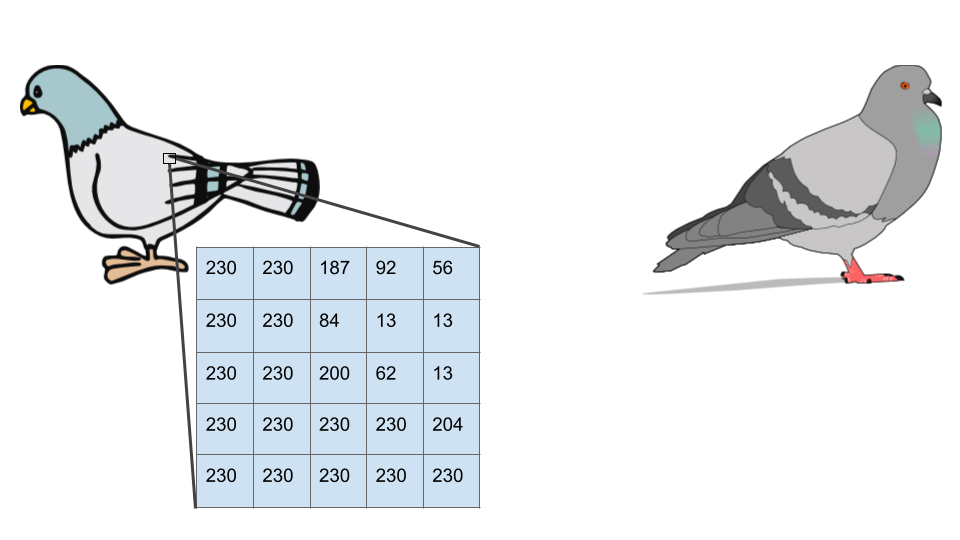
\includegraphics[width=0.8\textwidth]{images/pigeon start.png}
\end{frame}

\begin{frame}{Сопоставление шаблона}
Можно искать определённый шаблон на картинке скользящим окном:
\begin{itemize}
    \item Через корреляцию шаблона и текущего положения окна.
    \item Или через квадрат разницы.
\end{itemize}

\centering
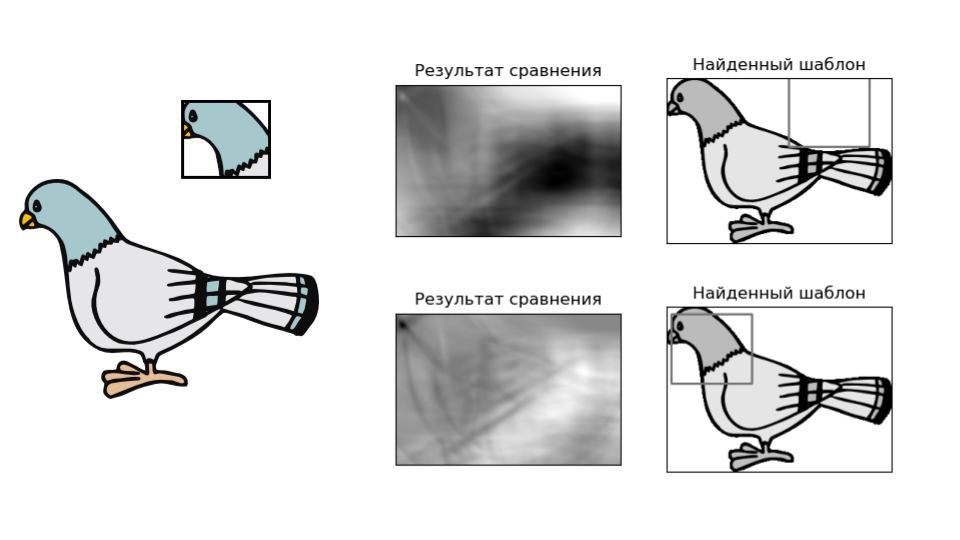
\includegraphics[width=0.8\textwidth]{images/pigeon template matching.png}

\alternativefootnote{\url{https://docs.opencv.org/master/d4/dc6/tutorial_py_template_matching.html}}
\end{frame}

\begin{frame}{Сопоставление шаблона}

\begin{itemize}
    \item Подправим способ сравнения, учтя общую освещённость.
    \item Для корреляции это помогло найти правильное местоположение.
\end{itemize}

\centering
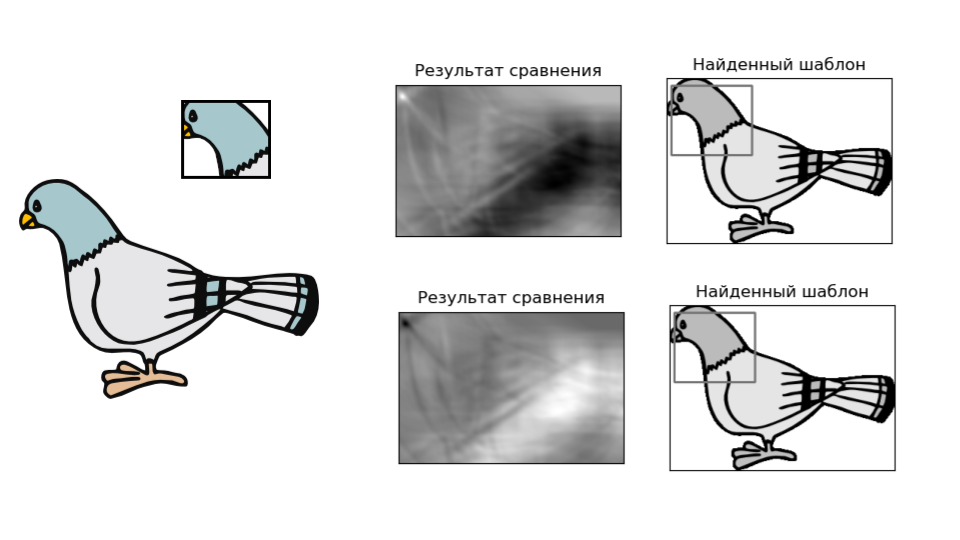
\includegraphics[width=0.8\textwidth]{images/pigeon template matching2.png}

\alternativefootnote{\url{https://docs.opencv.org/master/d4/dc6/tutorial_py_template_matching.html}}
\end{frame}


\section{Векторизация}

\subsection{Простая векторизация}

\begin{frame}{Глобальные статистики}

Какая глобальная информация о картинке может быть полезна для её поиска?

\begin{itemize}
    \item Гистограмма всех цветов (яркости).
    \item Переход в другое цветовое представление и гистограмма в нём.
    \item Применить преобразование Фурье, и смотреть статистики частот.
    \item Выбрать набор текстур, и описывать картинки через наличие в них таких текстур.
\end{itemize}

А ещё...

\pause
\begin{itemize}
    \item Представить картинку как взвешенную сумму других картинок.
\end{itemize}
    
\end{frame}

\begin{frame}{Разложение на базис}
    
\end{frame}

\subsection{CNN как векторизатор}

\begin{frame}{Дескрипторы классификационной CNN}

\begin{itemize}
    \item Свёрточные нейросети умеют правильно классифицировать картинки.
    \item Внутреннюю информацию можно извлечь и использовать в качестве описания картинки!
\end{itemize}

\centering
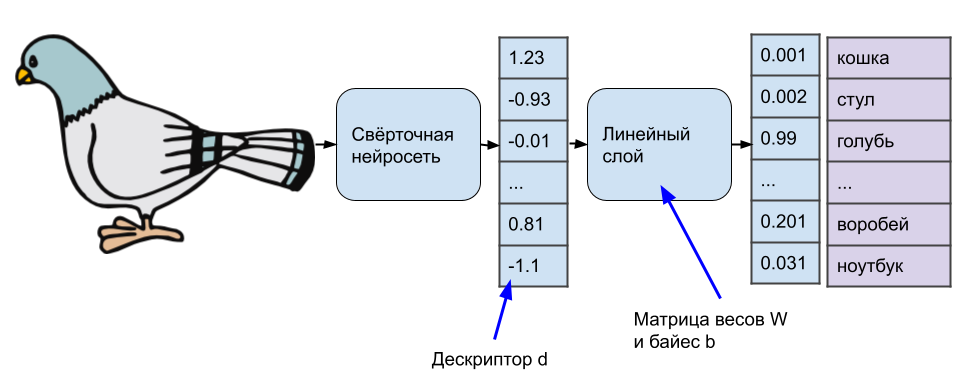
\includegraphics[width=0.8\textwidth]{images/pigeon CNN.png}

Итоговые предсказания класса $i$: $ \sigma_i(W^\Tr_i d + b_i) = \frac{\exp ( W^\Tr_i d + b_i )}{\sum_j \exp ( W^\Tr_j d + b_j )}$
    
\end{frame}

\begin{frame}{Вспоминаем задачу классификации}

Мы пытаемся минимизировать кроссэнтропию:
\[
CE(X,\,Y) = - \frac{1}{B} \sum_{k=1}^{B} \ln \frac{e^{W_{y_k}^\Tr d_k + b_{y_k}}}{ \sum_{j=1}^{N} e^{ W_{j}^\Tr d_k + b_{j} } } \rightarrow \min_{W,\,b,\,d}
\]

Сконцентрируемся только на одном объекте класса $i$:

\[
- \ln \frac{e^{W_{i}^\Tr d + b_i}}{ \sum_{j=1}^{N} e^{ W_{j}^\Tr d + b_{j} } } = 
\ln \left( \sum_{j=1}^{N} e^{ W_{j}^\Tr d + b_{j} } \right) - \ln e^{W_{i}^\Tr d + b_i} = 
\ln \left( \sum_{j=1}^{N} e^{ W_{j}^\Tr d + b_{j} } \right) - \left( W_{i}^\Tr d + b_i \right)
\]

Мы хотим, чтобы дескриптор $d$ был похож на столбец $W_i$ больше, чем на другие столбцы!
    
\end{frame}


\subsection{Обучение метрики}

\begin{frame}{Сиамские сети, обучения по парам}
\centering
\begin{tabular}{m{15em} m{10em}}
    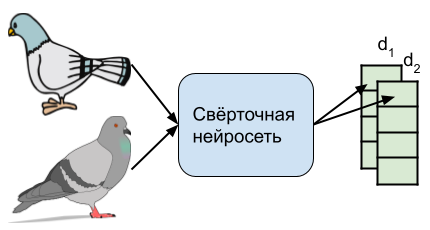
\includegraphics[width=0.38\textwidth]{images/siamse pigeon1.png} & 
    $
    \min_{d_1,\,d_2} \left( 1 - \frac{ d_1^\Tr d_2 }{\|d_1\|_2 \|d_2\|_2} \right)
    $
    \\
    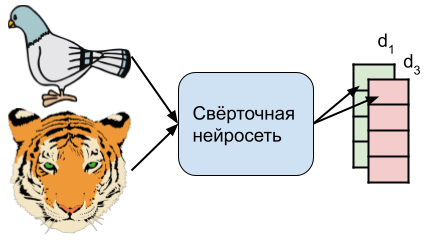
\includegraphics[width=0.38\textwidth]{images/siamse pigeon2.png} & 
    $
    \max_{d_1,\,d_3} \left( 1 - \frac{ d_1^\Tr d_3 }{\|d_1\|_2 \|d_3\|_2} \right)
    $
    \\
\end{tabular}

Если передавать метку $1$ для положительных пар и $-1$ для отрицательных, функцию ошибки можно записать в общем виде: $y_{ij} \left( 1 - \frac{ d_i^\Tr d_j }{\|d_i\|_2 \|d_j\|_2} \right) \rightarrow \min_{d_1,\,d_2}$

\end{frame}

\begin{frame}{Триплеты, схемы семплирования}

\begin{tabular}{m{14em} m{15em}}
    
\includegraphics[width=0.4\textwidth]{images/pigeon triplet1.png} &  
    --- случайное семплирование \\
    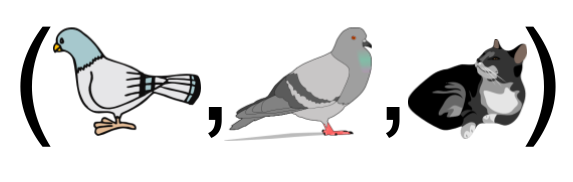
\includegraphics[width=0.4\textwidth]{images/pigeon triplet2.png} &  
    --- semi-hard negative sampling \\
    
\includegraphics[width=0.4\textwidth]{images/pigeon triplet3.png} &  
    --- hard negative sampling, hard positive sampling
\end{tabular}

Мы хотим, чтобы расстояние от якорного примера до положительного было меньше, чем до отрицательного.

Hinge loss: $ [ m + dist(d_A, d_P) - dist(d_A, d_N) ]_+ $
    
\end{frame}

\begin{frame}{Ещё обучения метрики}

\begin{itemize}
    \item Можно добавить пару к негативному примеру, получим квадруплеты!
    \item Можно пользоваться особенностью обучения по батчам, и семплировать примеры только изнутри батча.
    \item Используя матричные формы функции ошибки можно без семплирования оптимизировать сразу по всем возможным парам из батча.
    \item Можно формировывать псевдо-классы. И вместо отсемплированных примеров, брать эти псевдоклассы (Proxy-NCA).
    \item И ещё много идей...
\end{itemize}
    
\end{frame}

\begin{frame}{Но в реальности...}

Так всё это обучение метрик вообще помогает?

\begin{center}
    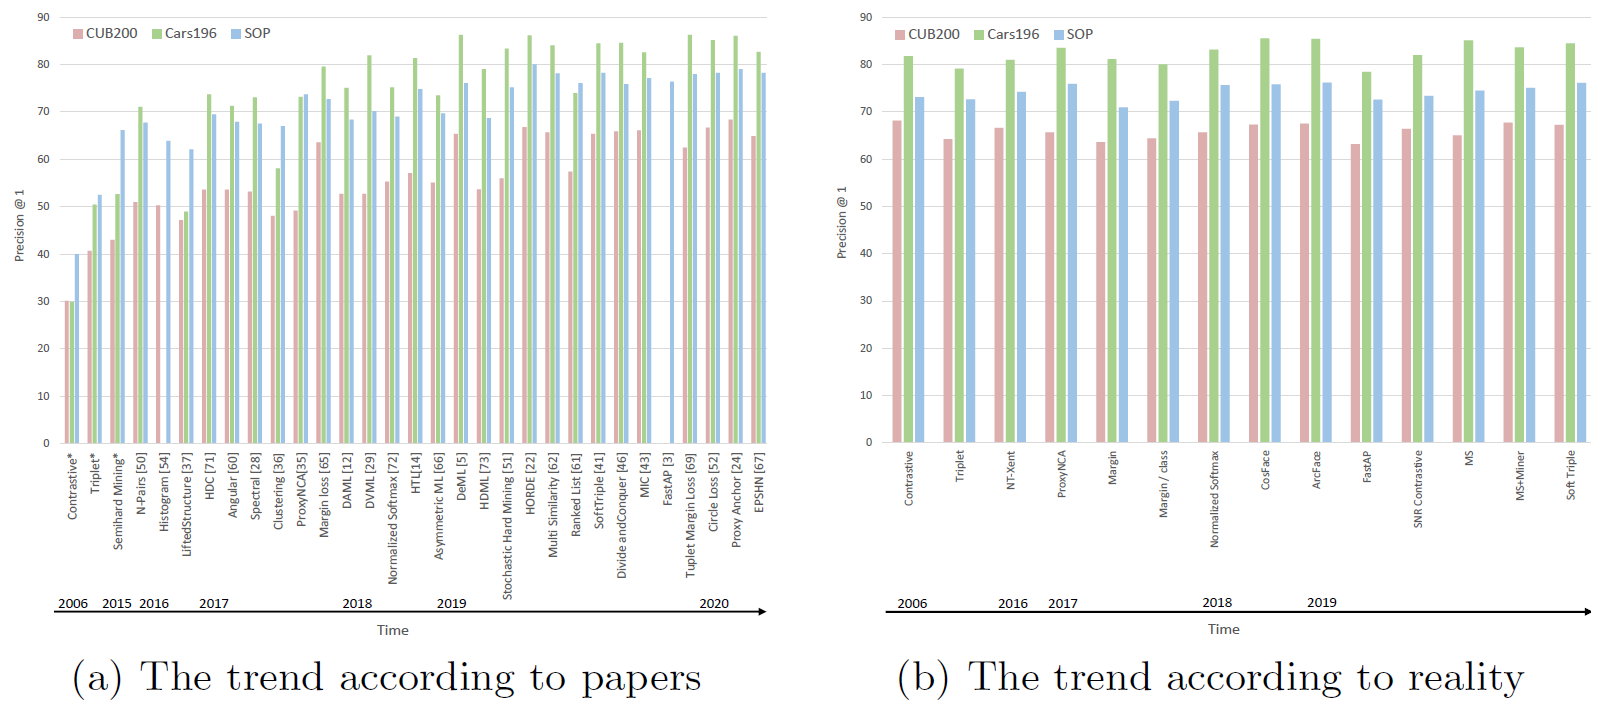
\includegraphics[width=0.9\textwidth]{images/reality check.png}
\end{center}

\alternativefootnote{\fullcite{musgrave2020metric}}
\end{frame}


\subsection{Angular Loss}

\begin{frame}{Минимизация угла}

Ещё раз про классификацию из дескриптора:
\[
\sigma_i(W^\Tr_i d + b_i) = \frac{\exp ( W^\Tr_i d + b_i )}{\sum_j \exp ( W^\Tr_j d + b_j )}
\]

Если мы отнормируем дескиптор $d$ и столбцы $W$, то скалярное произведение внутри экспоненты можно переписать:

\[
\frac{\exp ( \|W_i\|_2 \|d\|_2 \cos \theta_{i} + b_i )}{\sum_j \exp ( \|W_j\|_2 \|d\|_2 \cos \theta_{j} + b_j )} = \{ \|d\|_2 = 1,\, \|W_i\|_2 = 1 \} = 
\frac{\exp ( \cos \theta_{i} + b_i )}{\sum_j \exp ( \cos \theta_{j} + b_j )}
\]

В этом случае мы уменьшаем непосредственно угол между дескриптором и нужным столбцом матрицы $W$.
    
\end{frame}

\begin{frame}{Angular Loss}

А что если нам идею с зазором добавить в оптимизируемый нами угол?
\[
AngularLoss : \frac{e^{ \cos (m_1 \theta_{i} + m_2) + m_3} }{e^{ \cos (m_1 \theta_{i} + m_2) + m_3} + \sum_{j \neq i} e^{ \cos \theta_{j}} }
\]

\centering
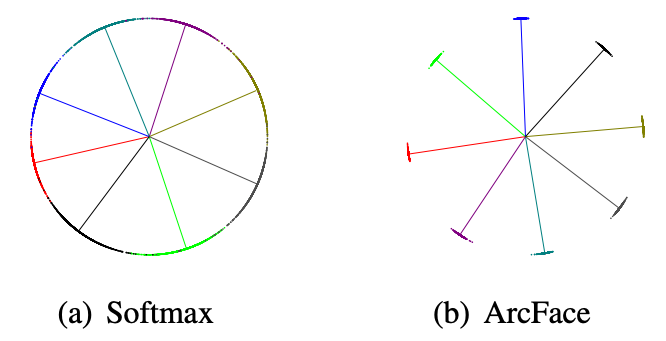
\includegraphics[width=0.5\textwidth]{images/arcface.png}
    
\end{frame}



\section{Локальные дескрипторы}

%\subsection{Простая векторизация}

\begin{frame}{Локальность признаков}

А что если мы векторизовывать будем не всё изображения, а его части?

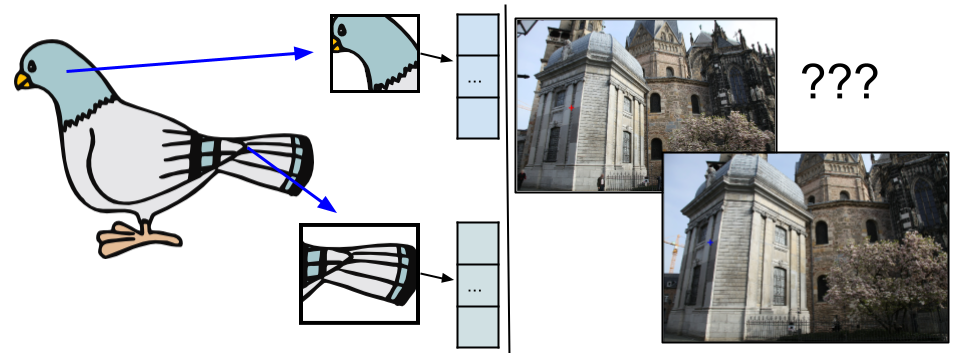
\includegraphics[width=0.9\textwidth]{images/pigeon local2.png}

Как понять, какие части изображения нам интересны?
    
\end{frame}

\begin{frame}{Особые точки}

\begin{itemize}
    \item Опишем набор особых точек: углы, локальные максимумы яркости, границы, и т.д.
    \item Теперь используя это описание будем искать такие наборы точек на нашем изображении.
\end{itemize}
\centering
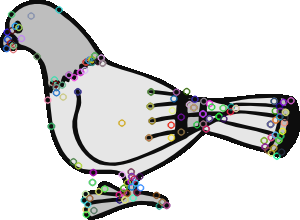
\includegraphics[width=0.3\textwidth]{images/pigeon_sift.png}
\end{frame}

\begin{frame}{SIFT-подобные дескрипторы}
Нам не достаточно находить только координаты.

\begin{tabular}{m{17em} m{20em}}
    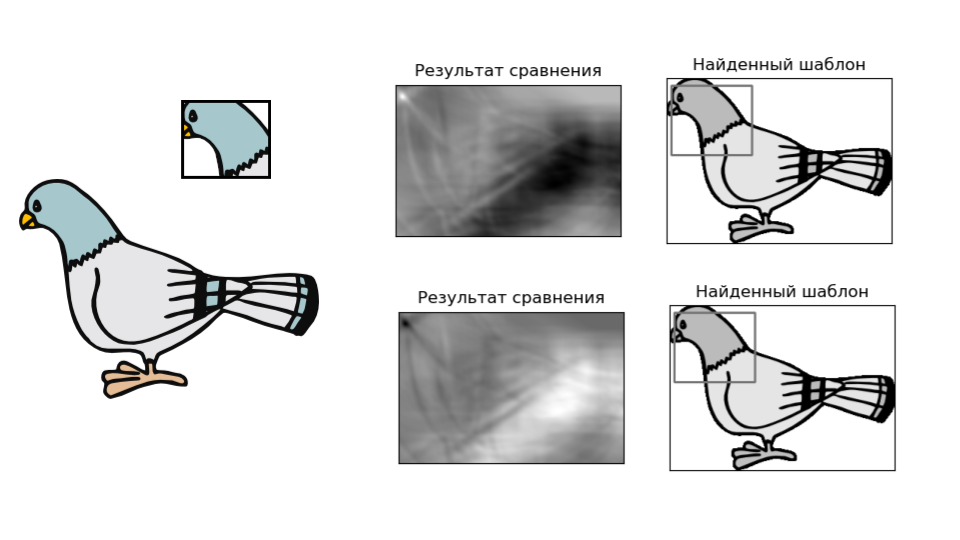
\includegraphics[width=0.5\textwidth]{images/pigeon template matching2.png} & 
    \begin{itemize}
        \item Можно использовать <<похожесть>> шаблона в качестве дескриптора точки.
        \item Ещё можно считать <<уникальность>> пикселя по сравнению с соседями.
    \end{itemize}
\end{tabular}
    
\end{frame}

\begin{frame}{Нейросети}

\begin{itemize}
    \item Если у нас есть фиксированный набор <<особенностей>>, можно обучить нейросетевой детектор.
    \item А затем дообучить его, чтобы на похожих точках он выдавал лизкие дескрипторы (SuperPoint\footfullcite{detone18superpoint}).
    \item У нас могут получиться плохие дескрипторы, давайте дополнительно оценивать <<надёжность>> (R2D2\footfullcite{r2d2})
\end{itemize}

\centering
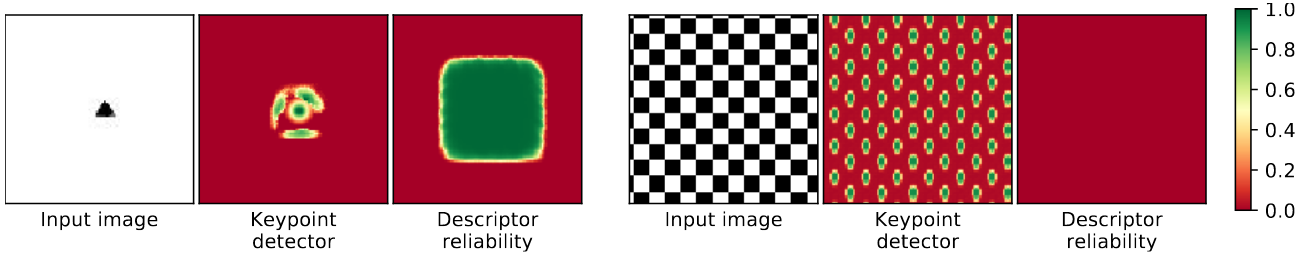
\includegraphics[width=0.9\textwidth]{images/r2d2_reliability.png}

\end{frame}

\begin{frame}{Матчинг дескрипторов}

\begin{itemize}
    \item Мы можем сравнивать дескрипторы как обычные вектора.
    \item Но чтобы сравнивать изображения надо сравнивать наборы дескрипторов друг с другом.
    \item При сравнении мы можем построить граф расстояний, и использовать его для дополнительной информации.
    \item Например обучить графовую нейросеть! (SuperGlue\footfullcite{sarlin20superglue})
\end{itemize}
    
\end{frame}


% \section{Ускорение поиска}

\subsection{Снижение размерности}

\begin{frame}{Снижение размерности}
    
\end{frame}

\begin{frame}{Quantization}
    
\end{frame}

\begin{frame}{Product Quantization}
    
\end{frame}

\subsection{Иерархические}

\begin{frame}{KD-деревья}
    
\end{frame}

\begin{frame}{Hierarchical Navigable-Small World}
    
\end{frame}


\section{Заключение}

\begin{frame}{Прочие способы поиска}

Можно улучшать поиск картинок, добавляя:
\begin{itemize}
    \item картинки того же объекта в разных положениях (аггрегация дескрипторов),
    \item мета-информацию об объекте (тэги, размеры),
    \item текстовое описание картинки или объекта,
    \item смешивая всё выше с разными весами (ансамблирование).
\end{itemize}
    
\end{frame}

% \begin{frame}{Так всё-таки как искать?}

% Важно понимать, что хотим искать
    
% \end{frame}

\begin{frame}{Что осталось за рамками}

\begin{itemize}
    \item Построение базы векторов.
    \item Инвертированный индекс (и мульти-индекс).
    \item Ускорение поиска ближайшего соседа внутри базы.
    \item Смешанные схемы по ускорению поиска ближайшего соседа.
    \item Нейросетевые подходы для поиска приближённого ближайшего соседа.
\end{itemize}
    
\end{frame}


\begin{frame}[plain]

\centering \Huge
Спасибо за внимание!

\vspace{17mm}
\Large
\begin{tabularx}{50mm}{Xl}
      \noindent\parbox[c]{\hsize}{
          
\includegraphics[width=7mm]{images/ods.png}
      }
      & @vuvko \\
      \noindent\parbox[c]{\hsize}{
          
\includegraphics[width=7mm]{images/1200px-Telegram_2019_Logo.png}
      }
      & @vuvko \\
      \noindent\parbox[c]{\hsize}{
          
\includegraphics[width=7mm]{images/GitHub-Mark-120px-plus.png}
      }
      & vuvko \\
      \noindent\parbox[c]{\hsize}{
          
\includegraphics[width=7mm]{images/1920px-XMPP_logo.svg.png}
      }
      & vuvko@fmap.me \\
      \noindent\parbox[c]{\hsize}{
          
\includegraphics[width=7mm]{images/1200px-Gmail_Icon.png}
      }
      & vuvko@fmap.me
\end{tabularx}
    
\end{frame}

\end{document}
